%*****************************************
\chapter{Lösungsansatz}\label{ch:approach}
%*****************************************
Die vorliegende Arbeit lehnt sich methodisch an das User-Centered Design an. 
Die Abbildung \ref{fig:approach} stellt die einzelnen Schritte dar.
Es darf dabei nicht unerwähnt bleiben, dass sich die Methodik in den einzelnen Schritten an unterschiedliche Werkzeuge(Methoden) bedient.
Dieses Kapitel konzentriert sich auf die Anwendung der User-Centered Design Methodik zur Lösung der Problemstellung der Arbeit und präsentiert die ausgewählten Werkzeuge in jedem Schritt des nutzerzentrierten Entwicklungsprozesses.

\begin{figure}[h]
	\centering
    	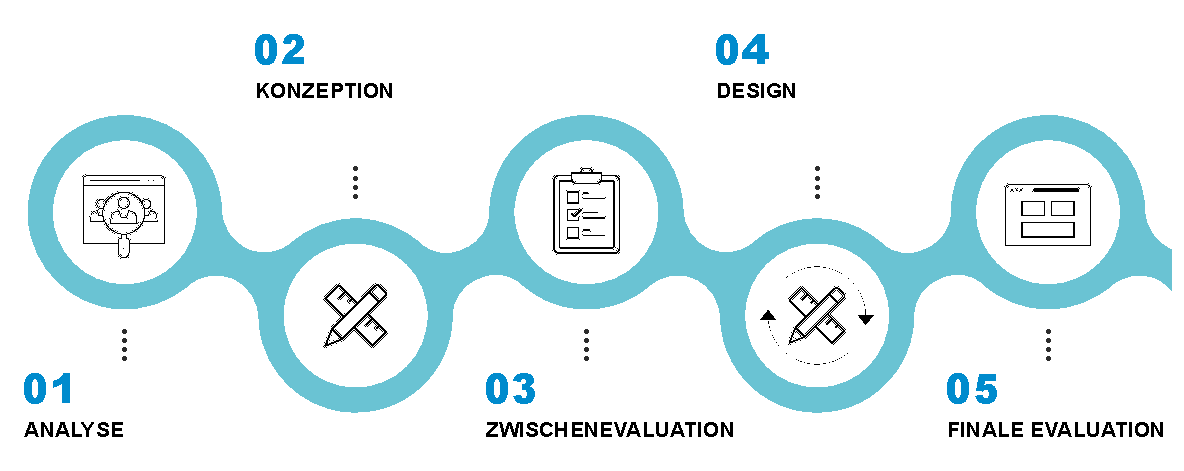
\includegraphics[width=0.95\textwidth]{Images/Ansatz}
   	\caption{Prozessschritte}
   	\label{fig:approach}
\end{figure}

\section{Analyse}

Der erste Schritt im Prozess der nutzerzentrierten Entwicklung ist die Durchführung einer Analyse.
Das Ziel der Analyse ist es den Nutzungskontext zu verstehen und beschreiben zu können.
Die aus der Analyse gewonnen Informationen werden im späteren Verlauf genutzt, um genaue Anforderungen definieren zu können.
Die nachfolgenden zwei Unterkapitel setzen sich mit den zwei ausgewählten Methoden zur Analyse im \ac{UCD}-Prozess auseinander.

\subsection{Befragung}\label{ch:interview}

Befragungen werden durchgeführt, um die Nutzeranforderungen zu erheben.
Ziel der Befragung ist sowohl die Datensammlung über mögliche Nutzer als auch Informationen über ihre Anforderungen an der neuen Darstellung der Wissensbasis und Einschätzungen zu der aktuellen Anwendung zu sammeln. 
Im Rahmen der vorliegenden Arbeit wird eine teilweise nicht standardisierte Befragung durchgeführt.
Es werden sowohl offene Fragen, als auch geschlossene Fragen gestellt.
Die offenen Fragen können in diesem Fall zu neue Erkenntnisse und Zusammenhänge führen.
Durch die geschlossenen Fragen, wird die aktuelle Lösung bewertet.
Die Ergebnisse der Befragung sollen als Basis der Definition von Personas im nächsten Schritt dienen.

\subsection{Personas}

Im Züge des Entwicklungsprozesses sollte man den Nutzer und seine Bedürfnisse stets im Blick behalten.
Aus diesem Grund werden mögliche Nutzer und deren Nutzverhalten in Form von Personas definiert.
Die gesammelten Daten aus der im Unterkapitel \ref{ch:interview} durchführten Befragung dienen zur Definition der Personas.
Personas sind fiktive Nutzer der Anwendung.
In dem vorliegenden Fall lassen sich drei unterschiedliche Persona-Typen identifizieren:

\begin{itemize}
	\item der \ac{CIO}
	\item die Arbeitskraft im Krankenhaus
	\item der Studierende
\end{itemize}

Diese drei Persona-Typen und deren Bedürfnisse werden im Laufe des nutzerzentrierten Entwicklungsprozesses im Mittelpunkt stehen.

\subsection{Ist-Analyse}



\section{Konzeption}\label{sec:concept}

Im zweiten Schritt des \ac{UCD}-Prozesses werden die Nutzungsanforderungen spezifiziert.
Hierbei wird die zugrundeliegende Informationsarchitektur und der User-Flow entwickelt.
Für diesen Schritt der nutzerzentrierten Entwicklung wurden Wireframes als Methode ausgewählt.
Wireframes konzentrieren sich ausschließlich auf den Aufbau der Seiten, die dargestellten Inhalte und die Interaktionsmöglichkeiten der Nutzer.

\section{Design}

Der dritte Schritt im \ac{UCD}-Prozess ist die Entwicklung der Gestaltungslösung.
Anhand der durchgeführten Analyse und des erstellten Konzeptes soll die Visualisierung der Anwendung verfeinert werden.
In diesem Schritt werden Methoden wie Mockups und Prototypen eingesetzt.
Im folgen werden die zwei Methoden präsentiert und deren Auswahl wird begründet.

\subsection{Mockups}\label{sec:mockup}

Bei dieser Methode werden die im Unterkapitel \ref{sec:concept} erstellten Wireframes zu detaillierte Screens ausgearbeitet.
Hierbei werden dann die Designkonzepte, wie zum Beispiel Farben, Typografie oder Bilder visualisiert.

\subsection{Prototypen}

Mit Hilfe von einem Protoytpen werden einzelne Teile der Anwendung simuliert.
Als Grundlage werden in diesem Schritt die im Unterkapitel \ref{sec:mockup} resultierende Mockups verwendet.

\section{Evaluation}

Der vierte und letzte Schritt der nutzerzentrierten Entwicklung sieht die Evaluation der entwickelten Lösung hervor.
Dabei wird die erarbeitete Gestaltungslösung anhand der Anforderungen getestet.
Somit können mögliche Probleme oder Hindernisse entdeckt und gelöst werden.
Aus zeitlichen Gründen wurde für diesen Schritt die Usability Review-Methode ausgewählt.
